\section{Algorithm Design and Data Structures}
\label{ch:alg}

\subsection{Identification of Critical Operations}
Ten operations decide correctness and performance: (1) neighbour discovery and link-quality estimation; (2) link-state dissemination; (3) least-cost route computation; (4) the per-packet forwarding decision; (5) priority scheduling; (6) duplicate suppression; (7) send, acknowledge and retry; (8) bounded store-and-forward; (9) encryption and signing; (10) resolution of the symbolic destination \texttt{RESCUE\_\_}. They correspond to Algorithms 1--10 of the Phase~II \emph{Design of Algorithms}; the pseudocode below reflects the implemented code, including the Phase~4 corrections.

\subsection{Algorithm Design}
\label{sec:algdesign}
\textbf{A1 Discovery and link quality.}
\begin{lstlisting}
every 3 s: broadcast HELLO(role, public_key)                      // ttl = 1
on HELLO from p:  new <- table.update(p);  if new: on_peer_up(p)
    q <- hellos_received / hellos_expected   in a 20-slot window    // in [0,1]
    if |q - last_reported| >= 0.1: report q                         // avoids recomputing on noise
every 1 s: for p silent > 10 s: remove p; on_peer_down(p)
\end{lstlisting}
A new neighbour is scored over the HELLOs \emph{due} so far, otherwise every fresh link would look lossy. (The Phase~II write-up planned a 10-slot window; the code uses 20.)

\textbf{A2 Link-state with re-flooding.}
\begin{lstlisting}
every 5 s: seq++; send report(origin=me, seq, [(p, q, failures, role, key) for p in neighbours]) to each neighbour
on report(origin, s, entries) from sender:
    if origin = me or s <= seq_seen[origin]: return                  // stale or own: stop
    seq_seen[origin] <- s;  replace origin's outgoing edges with entries;  learn roles and keys
    if changed: invalidate route cache
    forward report unchanged to every neighbour except origin and sender   // controlled re-flooding
\end{lstlisting}
Without re-flooding a node knows only its neighbours' neighbours; sequence numbers admit each report once per link, so flooding terminates.

\textbf{A3 Dijkstra and the cost function.}\label{sec:cost}
\begin{lstlisting}
cost(u->v) = 1 + 5 * (1 - q) + 3 * f        // f = ACK timeouts on the link in the last 60 s
dist[src] <- 0; heap <- {(0, src)}
while heap: (d,u) <- pop_min; if u visited: continue; mark u
    for (v, e) in graph.neighbours(u): if d + cost(e) < dist[v]: dist[v] <- d + cost(e); prev[v] <- u; push
next_hop(dst) = path[1] of the cached shortest path, or none (=> store-and-forward)
\end{lstlisting}
\textbf{Derivation of the coefficients.} The base 1 is the per-hop penalty; it keeps every weight positive (Dijkstra's condition) and prefers fewer hops between equal links. The term $5(1-q)$ makes loss expensive: a link delivering 40\,\% of its HELLOs costs $1+5(0.6)=4.0$, more than two clean hops (2.0) or three (3.0), which is exactly where minimum-hop routing errs (Figure~\ref{fig:cost}). The term $3f$ is steeper than the estimated-loss term because an ACK timeout is \emph{observed} failure: one adds the cost of three extra clean hops, and it applies at once so the retry avoids the failing link.
\begin{figure}[!htbp]
\centering
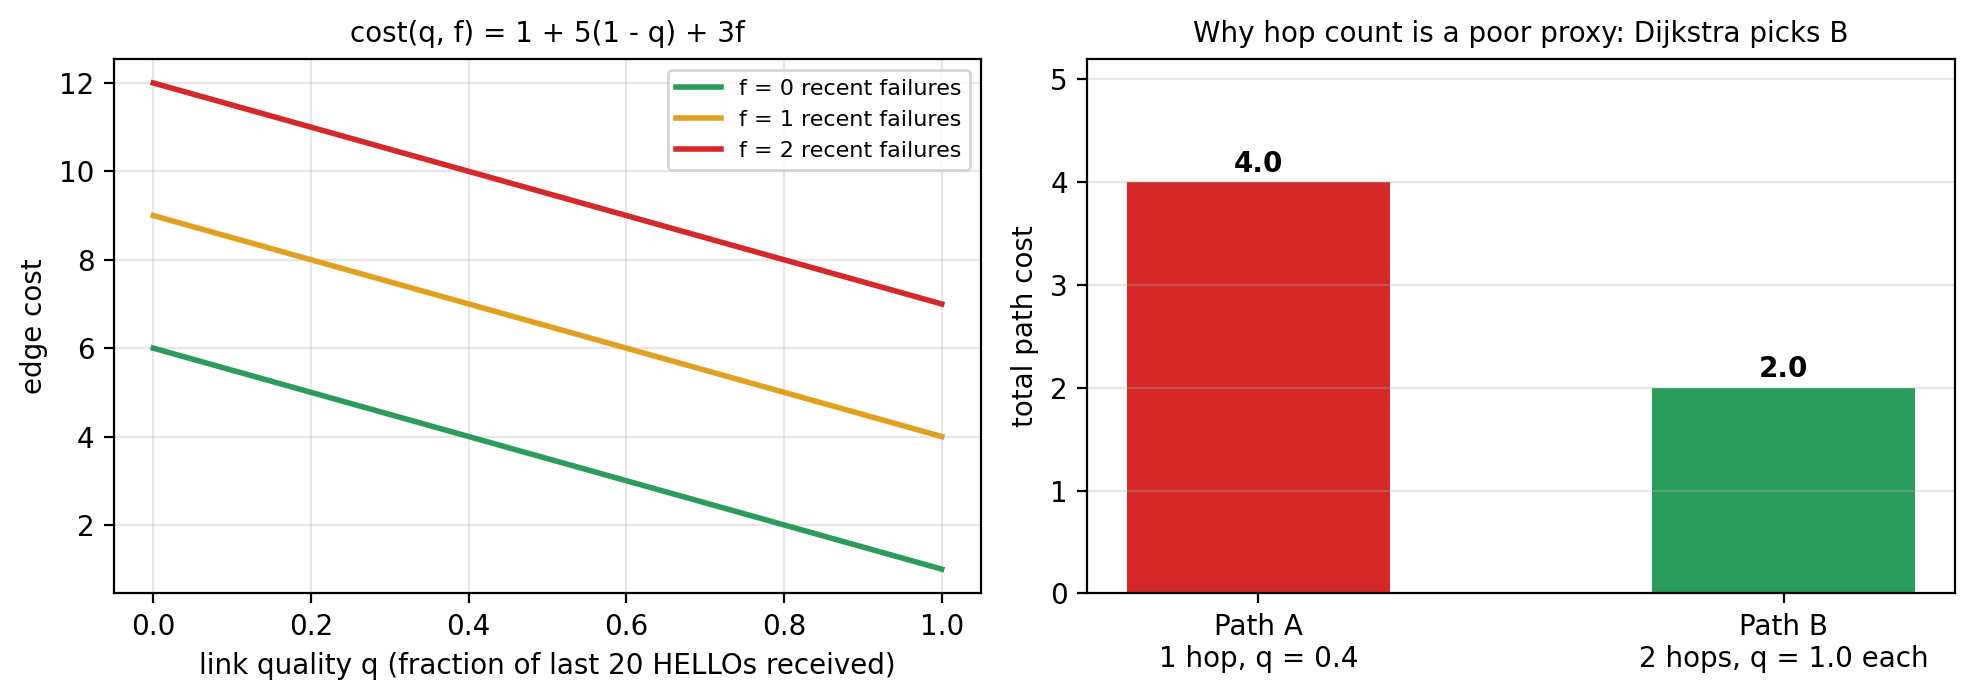
\includegraphics[width=0.5\textwidth]{figures/fig_cost.png}
\caption{The cost function, and why hop count is a poor proxy for delivery}
\label{fig:cost}
\end{figure}

\textbf{A4 Packet handling.}
\begin{lstlisting}
on packet p from link sender s:
    if not parse_ok(p) or p.type not in {DATA, ACK}: drop
    for_me <- p.dst = me or (p.dst = RESCUE__ and my role in {GATEWAY, RESCUE})
    key <- (type, msg_id) if for_me else (type, msg_id, attempt)     // a retry crosses relays that saw the original
    if dedup.seen_before(key): drop(duplicate); re-ACK if for_me; return
    if for_me: verify signature; decrypt; log; ACK if needs_ack; deliver
    elif ttl <= 0: drop(ttl_expired)   elif me in path: drop(loop)   elif no next_hop: drop(no_route)
    else: ttl--; hop_count++; path.append(me); queue.push(p, priority)            // A5
\end{lstlisting}
The key includes the \emph{type} because an ACK carries the id of the DATA it acknowledges (without it every ACK was dropped at the first relay the DATA had crossed, a bug found in integration), and the \emph{attempt} at relays so a retransmission is forwarded; at the destination the attempt is excluded so the application sees each message once. A relay with no route drops the packet and logs \texttt{no\_route}; only the originator retains (A8).

\textbf{A5 Priority scheduling.} \texttt{push} inserts (priority, timestamp, counter) into a binary heap and \texttt{pop} returns the highest priority, then the oldest; the counter prevents ties from comparing packets. Applied at \emph{every} hop, an SOS overtakes routine traffic repeatedly along the route. \textbf{A6 Dedup.} A hash map of keys to first-seen time, pruned after 300\,s. \textbf{A7 Send, ACK, retry.} Every 0.5\,s the tracker is polled; a timed-out packet with fewer than 3 attempts gets a failure recorded on its link (cost $+3$), a recomputed route and a resend; after 3 attempts it moves to store-and-forward (Figure~\ref{fig:flowsend}). \textbf{A8 Bounded store-and-forward.} \texttt{enqueue} evicts, when over 500 messages, the one with the largest (priority value, age), i.e.\ the lowest priority and oldest; \texttt{expire} drops anything older than 1800\,s regardless of priority; the flush (every 10\,s) sends each message whose destination now has a route. \textbf{A9 Security.} Send encrypts with a random nonce and signs the identity bytes; receive verifies against the sender's known key (an unknown signer is dropped) and then decrypts (a failed tag is dropped). \textbf{A10 \texttt{RESCUE\_\_}.} One Dijkstra run, then the nearest reachable node whose role is GATEWAY or RESCUE; none reachable means store-and-forward (Figure~\ref{fig:flowroute}).

\subsection{Flowcharts}
Figure~\ref{fig:flowsend} shows how a message is originated, acknowledged, retried and retained; Figure~\ref{fig:flowroute} shows how a next hop is chosen. The packet receive path is the activity diagram of Figure~\ref{fig:activity}.
\begin{figure}[!htbp]
\centering
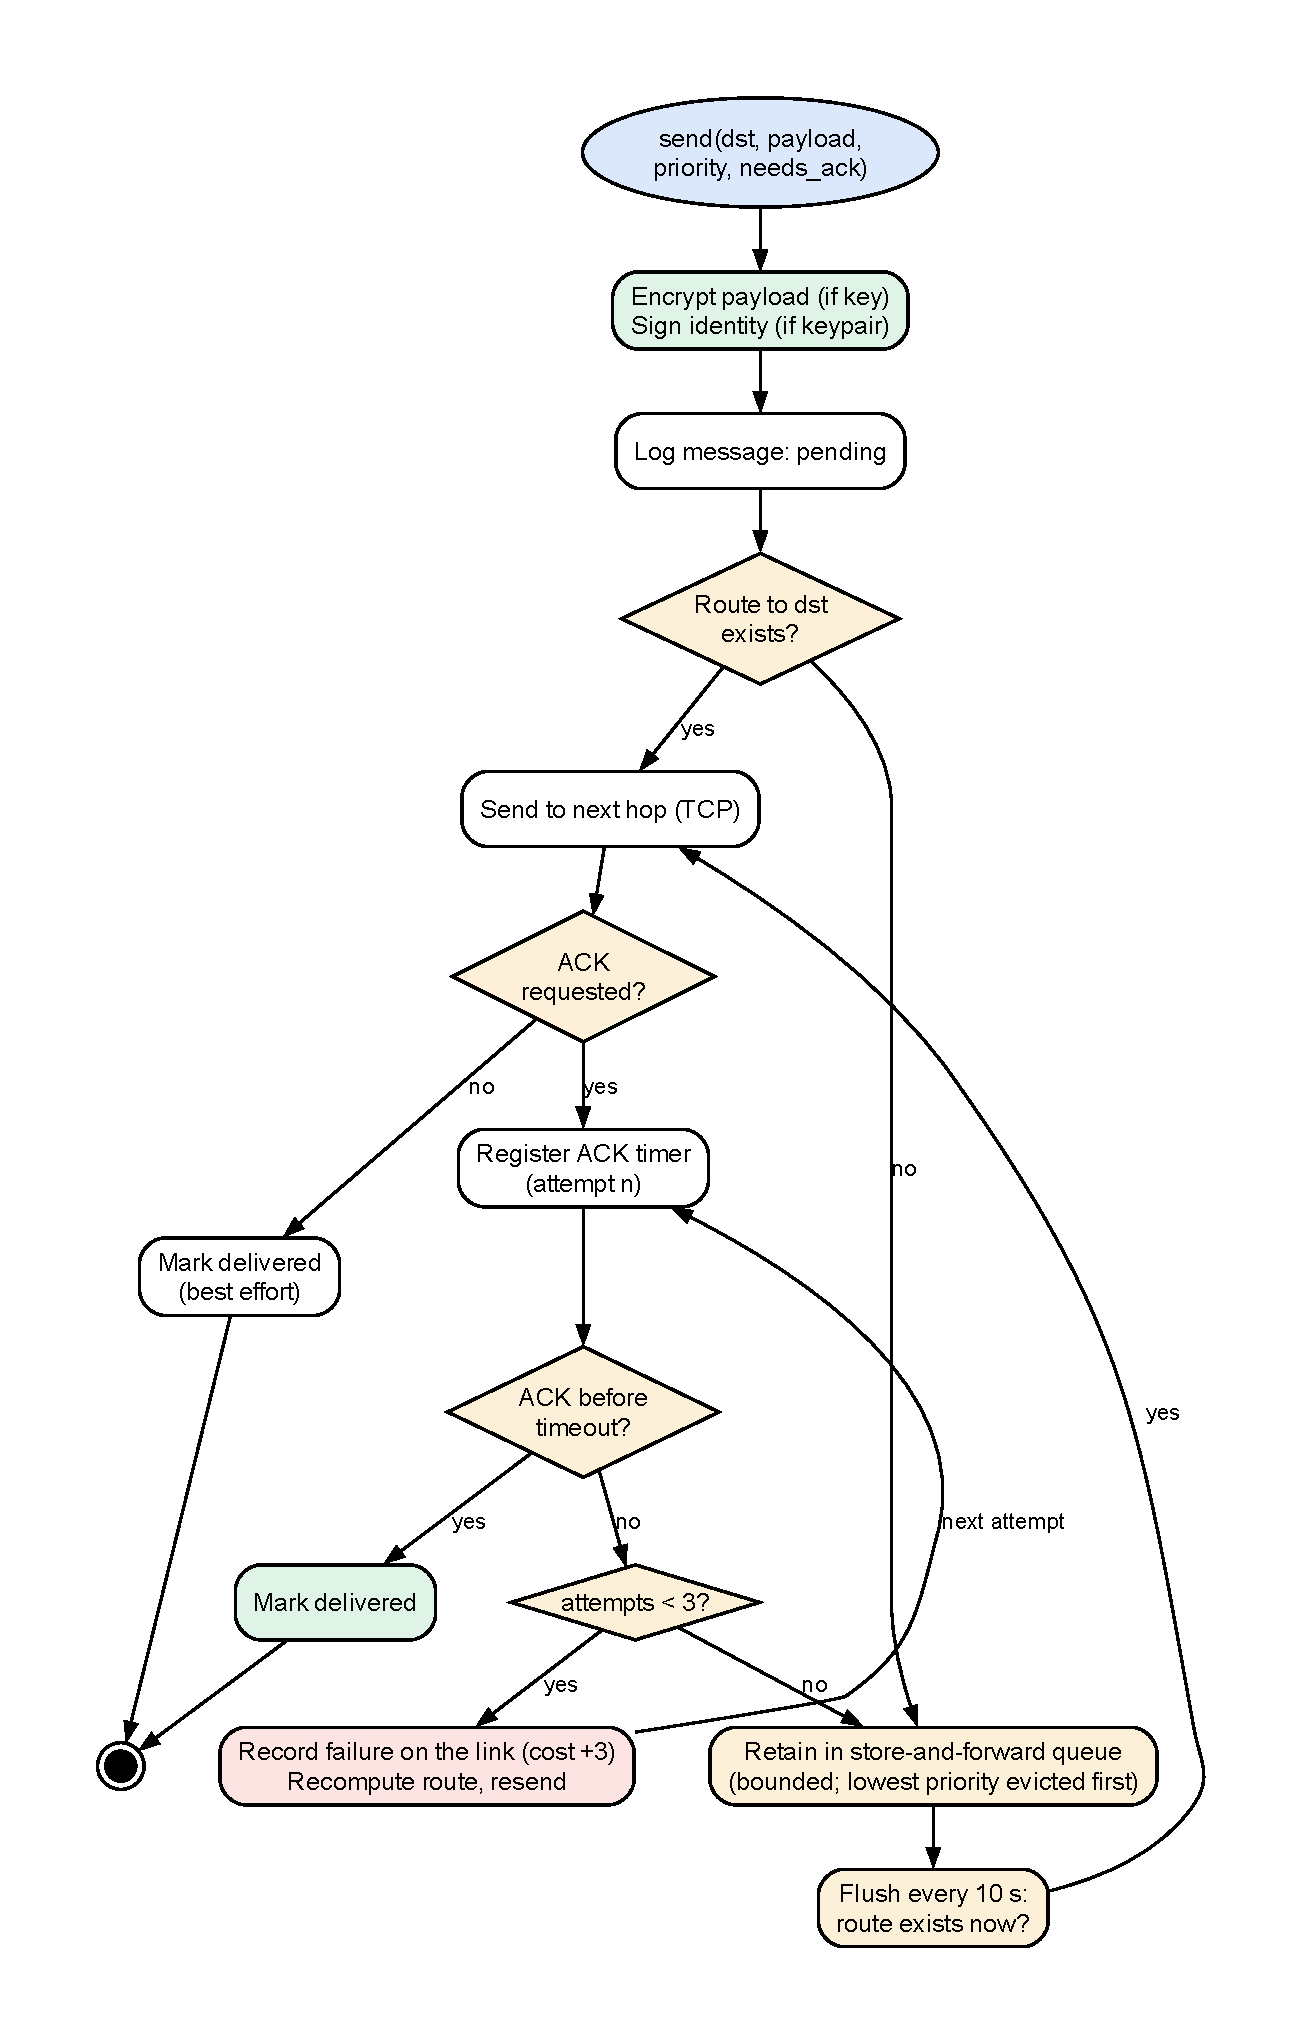
\includegraphics[height=0.36\textheight,keepaspectratio]{figures/fig_flow_send.pdf}
\caption{Flowchart: originate, acknowledge, retry and retain a message}
\label{fig:flowsend}
\end{figure}
\begin{figure}[!htbp]
\centering
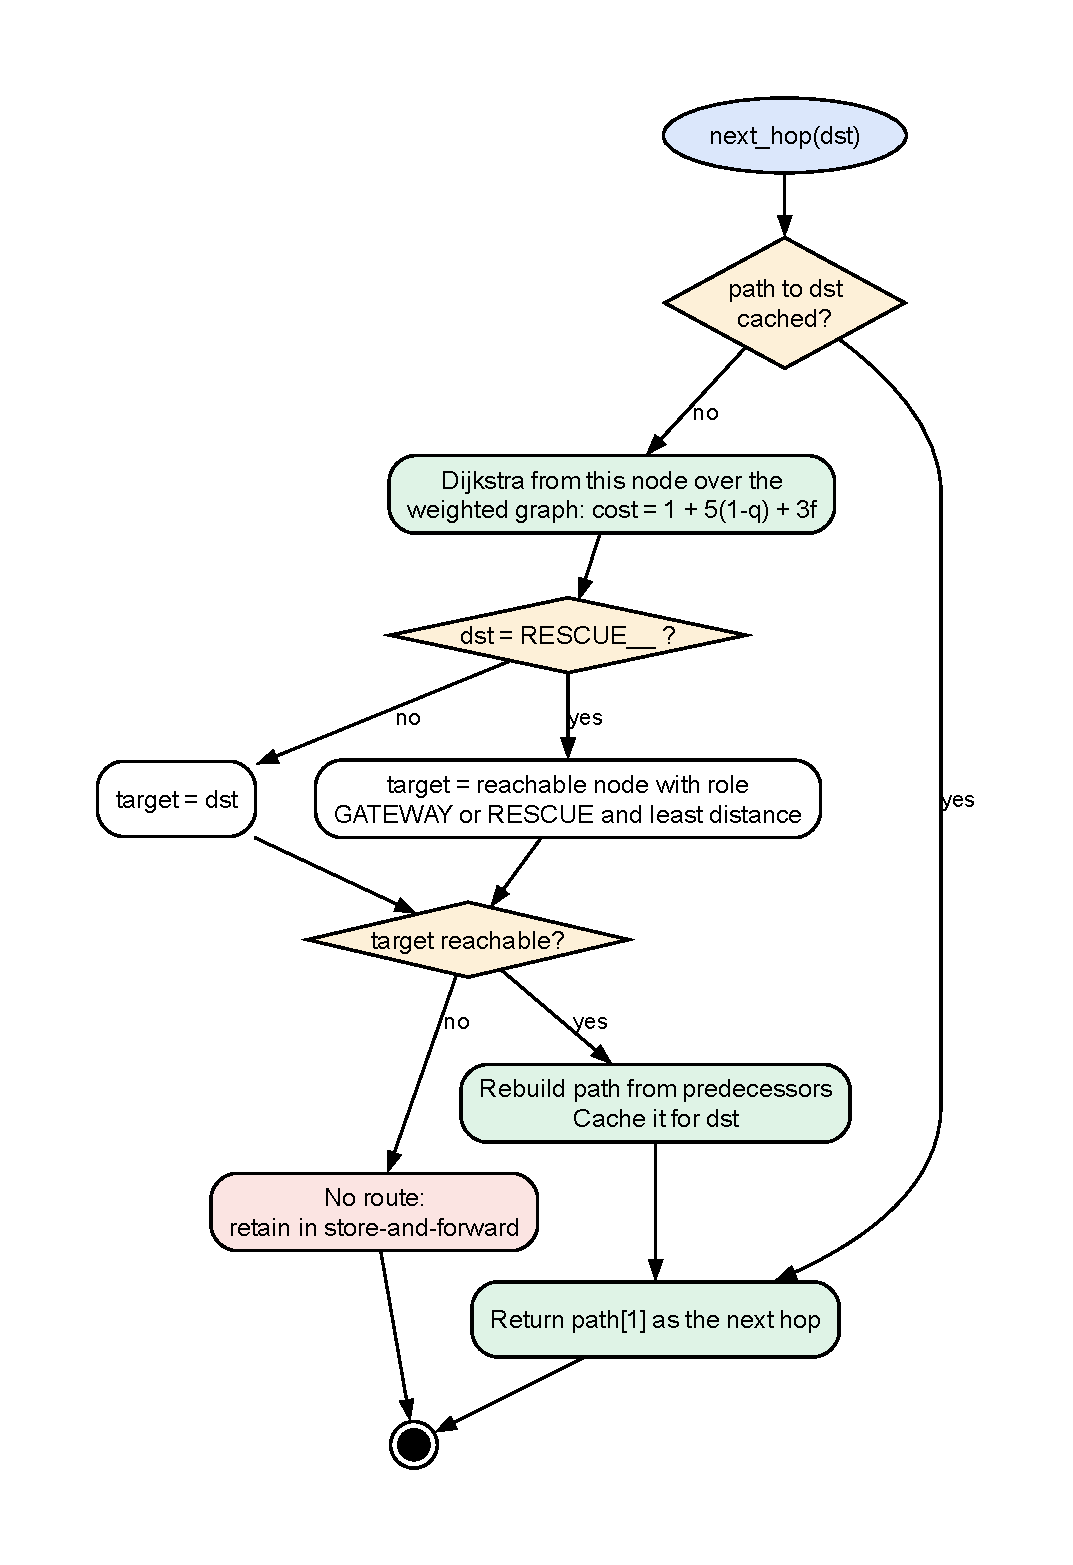
\includegraphics[height=0.32\textheight,keepaspectratio]{figures/fig_flow_route.pdf}
\caption{Flowchart: next-hop selection, including \texttt{RESCUE\_\_}}
\label{fig:flowroute}
\end{figure}

\subsection{Data Structure Selection}
\begin{table}[!htbp]
\caption{Data structures and why they were chosen}
\label{tab:ds}
\footnotesize
\begin{tabularx}{\textwidth}{@{}>{\raggedright\arraybackslash}p{4.2cm}>{\raggedright\arraybackslash}X@{}}
\toprule
\textbf{Structure and use} & \textbf{Reason}\\ \midrule
Adjacency dictionary of dictionaries: \texttt{MeshGraph} & $O(1)$ edge update and lookup, $O(\deg)$ iteration in Dijkstra; the mesh is sparse, so no matrix\\
Binary min-heap: Dijkstra frontier and the message priority queue & $O(\log n)$ insert and extract-min; ordering by (priority, timestamp, counter)\\
Hash map with timestamps: dedup set, neighbour table, route cache & $O(1)$ average membership; expiry by pruning\\
Fixed-capacity deque (20 slots) per neighbour & bounded sliding window for the link-quality estimate\\
Dictionary keyed by message id: ACK tracker, retention queue & $O(1)$ acknowledge and removal\\
Set: visited nodes in Dijkstra, reachable set & $O(1)$ membership\\
\bottomrule
\end{tabularx}
\end{table}

\subsection{Algorithm Selection and Justification}
Flooding delivers, but its message count grows with the square of the node count and it collapses a mesh under load. Bellman--Ford tolerates negative weights, which never occur here, at $O(VE)$; A* needs a geometric heuristic that a building mesh lacks. Dijkstra with a binary heap is correct for non-negative weights and runs in $O((V+E)\log V)$. Hop count, the default metric of the surveyed protocols, picks lossy shortcuts (Chapter~\ref{ch:perf} measures the difference). A sorted list would make insertion $O(n)$ and a FIFO cannot express priority; a hash set gives $O(1)$ duplicate checks where a list gives $O(n)$ on the hot path. The route cache is cleared on any topology change, which is simple and always correct.

\subsection{Time Complexity Analysis}
\begin{table}[!htbp]
\caption{Time complexity ($V$ nodes, $E$ links, $n$ queued packets, $q$ retained messages, $D$ distinct destinations, $|N|$ neighbours)}
\label{tab:complexity}
\footnotesize
\begin{tabularx}{\textwidth}{@{}>{\raggedright\arraybackslash}p{5.8cm}>{\raggedright\arraybackslash}X@{}}
\toprule
\textbf{Operation} & \textbf{Time}\\ \midrule
Dijkstra with the weighted cost & $O((V+E)\log V)$ in every case\\
Link-state merge on receiving a report & $O(\deg(v))$ plus $O(|N|)$ to re-flood\\
HELLO handling & $O(1)$ amortised\\
Priority enqueue / dequeue & $O(\log n)$; draining $n$ packets $O(n\log n)$\\
Duplicate detection & $O(1)$ average\\
Loop check & $O(|\text{path}|)$, at most 10 here\\
Store-and-forward flush & $O(D\,(V+E)\log V+q)$ with the route cache; worst case $O(q\,(V+E)\log V)$\\
Eviction & $O(q)$ scan, only when over the bound\\
Packet parse and validate & $O(1)$ for the fixed 52-byte header\\
\bottomrule
\end{tabularx}
\end{table}
Dijkstra's bound holds for every input. The cache makes repeated lookups to a destination $O(1)$ until a topology change clears it.

\subsection{Space Complexity Analysis}
Per node the graph needs $O(V+E)$ (a few hundred entries at 50 nodes), the dedup set is proportional to the traffic in the 300\,s window, the retention queue is bounded at 500 packets, and the neighbour windows hold $|N|\times 20$ timestamps. Dijkstra needs $O(V)$ extra for distances, predecessors and the heap. The SQLite log grows with the number of events and is the only unbounded structure; it lives on disk, not in memory.

\subsection{Optimization Opportunities}
\label{sec:opt}
Per-destination route-cache invalidation and incremental shortest paths instead of clearing the whole cache; multipoint relays to cut redundant copies of a report~\cite{rfc3626olsr}; short retention at relays (a relay with no route now drops the packet); batched SQLite commits (each event commits, which is safe but limits the logging rate); and the timer changes that the measurements point to (Chapter~\ref{ch:perf}).
